\documentclass{scrbook} % <= Druckversion: "scrbook", Bildschirmversion: "scrreprt"
\newcommand\bcor{12mm} % <= Bindungskorrektur für Druckversion
\usepackage{osm-thesis}

\usepackage{ellipsis} % Leerraumoptimierung
\usepackage{microtype}
\usepackage{enumitem} % Aufzählungen mit A, B, C ...
\usepackage{subcaption}

\usepackage[multiple]{footmisc} % Trennung mehrerer Fußnoten durch Kommata
% Requires \usepackage[hyperfootnotes=false,...]{hyperref}, see https://tex.stackexchange.com/a/35060

%%%%%%%%%%%%%%%%%%%%%%%%%%%%%%%%%%%%%%%%%%%%%%%%%%%%%%%%%%%%%%%%%%
% Tabellen
\usepackage{booktabs} % Tabellenstriche unterschiedlicher Stärke
\usepackage{tabularx} % Automatische Zeilenumbrüche
\usepackage{tablefootnote}
\newcolumntype{L}{>{\raggedright\arraybackslash}X}% Linksbündige Spalte ohne Trennung
\newcommand{\ra}[1]{\renewcommand{\arraystretch}{#1}}

%%%%%%%%%%%%%%%%%%%%%%%%%%%%%%%%%%%%%%%%%%%%%%%%%%%%%%%%%%%%%%%%%%
% Quellcode
\usepackage{minted} % Farbige Hervorhebung von Quellcode
\RequirePackage{csquotes} % Loaded later because of minted

%%%%%%%%%%%%%%%%%%%%%%%%%%%%%%%%%%%%%%%%%%%%%%%%%%%%%%%%%%%%%%%%%%
% Keine Einrückung nach Aufzählungen
\usepackage{etoolbox}
\makeatletter
\newcommand*\NoIndentAfterEnv[1]{%
	\AfterEndEnvironment{#1}{\par\@afterindentfalse\@afterheading}}
\makeatother

\NoIndentAfterEnv{enumerate}
\NoIndentAfterEnv{itemize}
\NoIndentAfterEnv{description}
\NoIndentAfterEnv{verse}
\NoIndentAfterEnv{minted}

%%%%%%%%%%%%%%%%%%%%%%%%%%%%%%%%%%%%%%%%%%%%%%%%%%%%%%%%%%%%%%%%%%
% Verzeichnisbäume
\usepackage[edges]{forest}

\definecolor{folderbg}{RGB}{124,166,198}
\definecolor{folderborder}{RGB}{110,144,169}
\newlength\Size
\setlength\Size{4pt}

\tikzset{%
	folder/.pic={%
		\filldraw [draw=folderborder, top color=folderbg!50, bottom color=folderbg] (-1.05*\Size,0.2\Size+5pt) rectangle ++(.75*\Size,-0.2\Size-5pt);
		\filldraw [draw=folderborder, top color=folderbg!50, bottom color=folderbg] (-1.15*\Size,-\Size) rectangle (1.15*\Size,\Size);
	},
	file/.pic={%
		\filldraw [draw=folderborder, top color=folderbg!5, bottom color=folderbg!10] (-\Size,.4*\Size+5pt) coordinate (a) |- (\Size,-1.2*\Size) coordinate (b) -- ++(0,1.6*\Size) coordinate (c) -- ++(-5pt,5pt) coordinate (d) -- cycle (d) |- (c) ;
	},
}
\forestset{%
	declare autowrapped toks={pic me}{},
	pic dir tree/.style={%
		for tree={%
			folder,
			font=\ttfamily,
			grow'=0,
		},
		before typesetting nodes={%
			for tree={%
				edge label+/.option={pic me},
			},
		},
	},
	pic me set/.code n args=2{%
		\forestset{%
			#1/.style={%
				inner xsep=2\Size,
				pic me={pic {#2}},
			}
		}
	},
	pic me set={directory}{folder},
	pic me set={file}{file},
}

%%%%%%%%%%%%%%%%%%%%%%%%%%%%%%%%%%%%%%%%%%%%%%%%%%%%%%%%%%%%%%%%%%
% Import SVG directly via Inkscape-pdf_tex-Export
\pdfsuppresswarningpagegroup=1
\usepackage{import}
\graphicspath{{images/}}
\newcommand{\executeiffilenewer}[3]{%
	\ifnum\pdfstrcmp{\pdffilemoddate{#1}}%
	{\pdffilemoddate{#2}}>0%
	{\immediate\write18{#3}}\fi%
} 
\newcommand{\includesvg}[1]{%
	\executeiffilenewer{#1.svg}{#1.pdf}%
	{inkscape -z -D --file=#1.svg %
		--export-pdf=#1.pdf --export-dpi=72 --export-latex}%
	\input{#1.pdf_tex}%
}
%%%%%%%%%%%%%%%%%%%%%%%%%%%%%%%%%%%%%%%%%%%%%%%%%%%%%%%%%%%%%%%%%%
% ABOUT
\newcommand{\hpitype}{Masterarbeit}
\newcommand{\hpiauthor}{Jan-Henrich Mattfeld}

% und Implementierung	
\newcommand{\hpititle}{%
	Entwurf einer %
	einheitlichen Middleware zur %
	Policy-Durchsetzung in %
	Multi-Cloud-Infrastrukturen}
\newcommand{\hpititleother}{Design and Implementation of a Unified Middleware for Policy Enforcement in Multi-Cloud Infrastructures} % <= das Studienreferat verlangt einen deutschen UND englischen Titel

\newcommand{\hpisupervisor}{Max Plauth, Prof.\,Dr.\,Andreas Polze}
\newcommand{\hpichair}{Fachgebiet für Betriebssysteme und Middleware}
\newcommand{\hpiexternalsupervisor}{}
\newcommand{\hpiexternal}{}
\newcommand{\hpidate}{\today}

% DOCUMENT
%\KOMAoption{draft}{true} % <= z.B. zum "Debuggen" der Overfull-Boxes und schnellerem Kompilieren https://tex.stackexchange.com/a/49369
\bibliography{literature/bibliography}

\begin{document}
	\selectlanguage{ngerman}

	% Einband
	\pagenumbering{alph}
	\ifisbook\include{content/coverpage}\fi
	\ifisbook\cleardoubleemptypage\fi

	% (Haupt-)Titelseite, Abstract, ggf. Danksagung & Inhaltsverzeichnis
	\pagenumbering{roman}
	\include{content/titlepage}
	\ifisbook\cleardoubleemptypage\fi
	 \null\vfil
\begin{otherlanguage}{ngerman}
\begin{center}\textsf{\textbf{\abstractname}}\end{center}

Cloud-Ressourcen spielen eine entscheidende Rolle in den aktuellen und zukünftigen IT-Strategien von Unternehmen aller Größen. Gleichzeitig entstehen zentrale Herausforderungen in Hinblick auf Vertraulichkeit und Zuverlässigkeit, sowie Portabilität der eigenen Daten und Anwendungen. Mit dem Inkrafttreten der Datenschutz-Grundverordnung und immer neuen Datenlecks ist das Thema hochaktuell.

Durch die intelligente Kombination von Private- und Public-Cloud-Infrastruktur treten wir diesen Herausforderungen entgegen. Wir geben einen Überblick über aktuelle kommerzielle und akademische Multi-Cloud-Projekte. Dabei identifizieren wir fehlende SLA- und Cloud-Schnittstellen-Standards als größte Risiken.

Als Lösungsvorschlag entwickeln wir einen Multi-Cloud-Anwendungs-Broker auf den Ebenen IaaS und CaaS. Dabei dient das TOSCA-Simple-Schema zur Anwendungs- und SLA-Spezi\-fi\-ka\-tion. Wir diskutieren den Aufwand der Cloud-Teststellungen und den Einsatz der Multi-Cloud-Bibliothek Apache Libcloud. Die Leistungsfähigkeit der Lösung demonstrieren wir anschließend in einem Testaufbau mit OpenStack, AWS, Docker und Hyrise-R.

Wir versetzen Cloud-Kunden in die Lage, ihre Anforderungen anbieter- und technikunabhängig zu formulieren und durchzusetzen. Unsere Lösung automatisiert die Einhaltung von Datenschutz-, Qualitäts- und Kostenzielen. Damit ist das Projekt einzigartig und ergänzt die bisherigen Beiträge im SSICLOPS-Kontext.

\end{otherlanguage}
\vfil\null




	\tableofcontents
	\cleardoublepage

	% Textteil
	\pagenumbering{arabic}
	\chapter{Einleitung}

Cloud-Angebote sind allgegenwärtig und werden mittlerweile von einer Mehrzahl deutscher Unternehmen genutzt. Laut \emph{Statista} setzten bis 2016 mindestens fünfundsechzig Prozent aller Betriebe entsprechende Lösungen ein \cite{bitkom:2017:cloud-nutzung-unternehmen}. Besonders gefragt sind Infrastrukturdienste, wie Rechenleistung und Speicher. Gleich darauf folgen Softwareangebote und E-Mail-Hosting. Etwas abgeschlagen bleiben Plattformdienste wie Datenbanken und Ausführungsumgebungen \cite{destatis:2016:cloud-nutzung-unternehmen-einsatzzweck}. Der Trend zur Cloud wird sich vermutlich fortsetzen: So vervierfacht sich das prognostizierte Marktvolumen mit Cloud-Services bis 2020 auf über sechzehn Milliarden Euro allein im deutschen B2B-Markt \cite{isg:2017:cloud-ausgaben-2020}.

Cloud-Angebote sind für Unternehmen aller Größen attraktiv: Die Anschaffung eigener Infrastruktur entfällt, genauso wie deren Wartung durch eigenes Personal. Stattdessen lassen sich Ressourcen und Anwendungen einfach per Self-Service buchen und sind anschließend über das Internet von überall erreichbar. Der Umfang gebuchter Leistungen lässt sich meist frei skalieren. Da die Angebote oft in kleinem Takt und verbrauchsgenau abgerechnet werden, ergeben sich so theoretisch Vorteile bei Flexibilität und Kosteneffizienz.

Demgegenüber stehen Vorbehalte bezüglich Datenschutz, denn die gemietete Infrastruktur teilen sich mehrere Kunden. Durch Sicherheitslücken wie \emph{Spectre} und \emph{Meltdown} werden eigentlich geschützte Speicherbereiche angreifbar \cite{Kocher2018spectre, Lipp2018meltdown}. Nach aktuellem Stand existierten diese Lücken mehr als ein halbes Jahr in fast jedem x86-System, und damit in fast jeder Cloud \cite{techcrunch:2018:spectre-meltdown-tier-2-cloud-vendors}. Eine sichere Mandantentrennung war also nicht mehr gewährleistet \cite{aws:2018:security-bulletin}. Aber auch durch Unachtsamkeit werden Cloud-Datenspeicher immer wieder der Öffentlichkeit zugänglich \cite{upguard:2017:breach-alteryx, upguard:2017:breach-centcom, kromtech:2018:breach-fedex}.

Zugleich fordert aktuelle Gesetzgebung wie die Datenschutz-Grundverordnung unter anderem die Verarbeitung von personenbezogenen Daten europäischer Kunden ausschließlich innerhalb der EU \cite{eu:2016:bdsvg}. Gut neunzig Prozent aller Unternehmen achteten folglich bei der Auswahl eines Cloud-Providers auf Rechts- und Server-Standorte in Deutschland \cite{gartner:2017:cloud-market}. Auch vorhandene Softwarelizenzen können den Umzug verhindern. Zum Beispiel Oracle- und Microsoft-OEM-Lizenzen verbieten die Übertragung in eine Cloud-Umgebung \cite{microsoft:2017:licensing, oracle:2018:licensing}. So müssen möglicherweise Teile der Infrastruktur lokal vorgehalten werden.

Für gut fünfzig Prozent der interessierten Unternehmen außerdem unabdingbar: individuelle Dienstgütevereinbarungen, sogenannte \emph{Service Level Agreements (SLAs)} \cite{bitkom:2017:cloud-nutzung-unternehmen-auswahlkriterien}. Dies lässt jedoch einige der weltweit größten Cloud-Anbieter außen vor -- Amazon und Microsoft teilen sich seit 2016 über fünfzig Prozent des weltweiten Umsatzes mit Infrastrukturdiensten \cite{gartner:2017:cloud-market}. Die Vertragsbedingungen beider Anbieter sind jedoch nicht verhandelbar.

Laut Gartner wollen daher 70 Prozent aller Unternehmen bis 2019 eine Multi-Cloud-Strategie umsetzen \cite{gartner:2017:cloud-market-multicloud-trend}. Auch das EU-geförderte Forschungsprojekt \emph{Scalable and Secure Infrastructures for Cloud Operations (SSICLOPS)} identifiziert Multi-Cloud-Umgebungen als zukünftigen Treiber des ITK-Markts \cite{ssiclops:2015:d6.1-project-presentation}. Zusätzlich zu einer privaten Cloud werden hierbei auch Dienste aus weiteren öffentlichen Angeboten genutzt. Vorteil ist eine höhere Flexibilität, um für jede Anforderung die ideale Cloud wählen zu können. Kriterien sind zum Beispiel die Einhaltung gesetzlicher Anforderungen, spezielle SLAs, höhere Ausfallsicherheit und die Preisgestaltung der Anbieter. Multi-Cloud birgt aber auch einige Herausforderungen:

\begin{itemize}
	\item Portabilität eigener Anwendungen
	\item Cloud-Provider-spezifisches Know-how
	\item Höherer IT-Verwaltungsaufwand der Ressourcen
	\item Managementaufwand, wie der Vergleich von Compliance-Richtlinien
	\item Keine oder geringere preisliche Skaleneffekte
	\item Überwachung der heterogenen Cloud-Landschaft
	\item Durchsetzung der eigenen Sicherheits- und Datenschutzrichtlinien
\end{itemize}

Um diese Herausforderungen automatisiert abzumildern, eignet sich eine \emph{Cloud-Management-Plattform (CMP)} mit integriertem Anwendungs-Broker. Deren Marktsituation ist allerdings unübersichtlich und in großer Bewegung. Bereits im letzten Jahr wurden einige vielversprechende Lösungen von Cloud-Infrastruktur-Providern aufgekauft \cite{gartner:2017:cloud-market-multicloud-trend}. Die CMPs sind nun selbst Software-as-a-Service-Angebote und proprietär. Die eigentlichen Vorteile Flexibilität und Unabhängigkeit werden so ad absurdum geführt.

Unabhängige Lösungen sind mehrheitlich ausgelaufene akademische Forschungsprojekte. Auf den aktuellen Cloud-Markt und technische Neuerungen wie Container sind diese nicht mehr anwendbar. Aufgrund der vorherigen Forschungsergebnisse ergibt sich jedoch folgende Hypothese:

\begin{verse}
	{\emph{Eine unabhängige, auf offenen Standards basierende CMP kann die \newline Vorteile der Cloud mit aktuellem Datenschutz vereinen.}}
\end{verse}

Im Rahmen dieses Projektes entwickeln wir einen Multi-Cloud-Broker. Alle Ergebnisse basieren auf Open-Source-Technologien und sollen, wenn möglich, an die Ursprungsprojekte zurückfließen. Der Broker soll Organisationen und Unternehmen als Cloud-Nutzer emanzipieren und besonders den kommerziellen Wert der Lösung herausstellen.

Da SLAs und weitere Rahmenbedingungen oft nicht verhandelbar sind, muss die Optimierung der Cloud-Nutzung in Eigenregie erfolgen.  Die vorgestellte CMP erlaubt die Nutzung bestimmter Anbieter, obwohl SLAs  nicht eingehalten werden: Zum Beispiel lässt sich eine höhere Ausfallsicherheit durch Kombination mehrerer Anbieter erreichen. Nebenbei entsteht so ein Notfallplan zum Weiterbetrieb bei Ausfall oder Kündigung eines Cloud-Providers.

Das folgende Kapitel klassifiziert Cloud-Angebote anhand bestimmter Eigenschaften und Service-Ebenen. Außerdem geben wir eine Einführung in datenschutzrechtliche Fragen und Risiken in Zusammenhang mit Cloud-Bereit\-stel\-lungs\-model\-len.

Anschließend entwickeln wir passende Policys und entsprechende Schemata. Diese sollen von dem eigens entwickelten Multi-Cloud-Broker verwendet werden. Er verteilt auch bestehende, nicht Cloud-native, Anwendungen über verschiedene Cloud-Provider auf IaaS- und CaaS-Ebenen und optimiert die Cloud-Landschaft anschließend fortlaufend. Dabei beachtet er SLAs und Datenschutzanforderungen. Für diesen Vorschlag bewerten wir akademische und kommerzielle Projekte mit ähnlicher Zielsetzung.

Der Implementierungsteil vergleicht verschiedene Multi-Cloud-Bibliotheken. Auf Basis von Apache \emph{Libcloud} entwickeln wir eine CMP, die das Multi-Cloud-Brokering übernimmt. Auch Implementierungshürden und Besonderheiten der verschiedenen Clouds werden beschrieben. Als Beispielanwendung dient dabei die verteilte Forschungsdatenbank \emph{Hyrise-R}. Auch die Entstehung eines \emph{OpenStack}-Testbeds als Beispiel einer Private-Cloud wird besprochen. Es folgt eine abschließende Bewertung des Konzepts.

	\chapter{Hintergrund -- Chancen und Herausforderungen in der Cloud}

Dieses Kapitel definiert die grundlegenden Charakteristika eines Cloud-Dienstes, die verschiedenen Service-Ebenen, Liefermodelle, Akteure und ihre Verantwortlichkeiten. Aus diesen Definitionen entwickeln sich zwei grundlegende Herausforderungen der Cloud-Nutzung:

\begin{enumerate}
	\item Datenschutz/Vertraulichkeit
	\item Portabilität von Daten und Anwendungen
\end{enumerate}

Je nach Cloud-Nutzung ergeben sich hierfür verschiedene Lösungsansätze, die im weiteren Verlauf gegeneinander abgegrenzt werden.


\section{Eigenschaften eines Cloud-Dienstes}

Unabhängig von Liefer- und Servicemodell zeichnet sich ein Cloud-Dienst durch bestimmte Merkmale aus. Konkret definieren übereinstimmend \emph{NIST Cloud Computing Reference Architecture}, \emph{IETF} und \emph{BSI-Grundschutzkatalog} \cite{nist:2011:reference-architecture, ietf:2015:reference-framework, bsi:2014:grundschutz} folgende Eigenschaften:

\begin{description}
	
	\item[On-demand Self-Service] Ressourcen werden vom Cloud-Kunden selbstständig über ein Portal oder eine Webschnittstelle angefordert und anschließend automatisch provisioniert.
	
	\item[Breitbandzugriff] Die gemieteten Ressourcen werden über ein Netzwerk, typischerweise das Internet, bereitgestellt. Der Zugriff erfolgt über Standardschnittstellen wie HTTP; kann also von überall erfolgen und ist im Regelfall nicht auf bestimmte Geräte oder Software beschränkt.
	
	\item[Geteilte Infrastruktur] Die zugrunde liegenden physischen Ressourcen werden virtualisiert und flexibel unter mehreren Kunden aufgeteilt. Die vorhandene Hardware wird so möglichst optimal ausgelastet. Gleichzeitig ergeben sich hierdurch Datenschutzbedenken; die Daten einzelner Mandaten müssen streng getrennt sein.
	
	\item[Elastizität] Durch einen hohen Grad an Automatisierung werden Ressourcen zeitnah zur Verfügung gestellt. Lastspitzen können ohne manuelle Eingriffe abgefangen werden.
	
	\item[Messbarkeit] Die Ressourcennutzung ist messbar und wird kontinuierlich überwacht. Abgerechnet wird zum Beispiel nach CPU-Zeit, Speicherkapazität oder Anzahl genutzter IP-Adressen.
	
\end{description}

Von klassischem IT-Outsourcing grenzt es sich durch Self-Service, Skalierbarkeit und geteilte Infrastruktur ab. Diese Eigenschaften bieten Kunden theoretisch Flexibilität und Kostenvorteile. In der Lösungssuche sollen diese positiven Aspekte möglichst erhalten bleiben.


\section{Service-Ebenen}

Je nach Auswahl des Cloud-Angebots lassen sich verschiedene Kernebenen unterscheiden. Diese bauen jeweils aufeinander auf und verbergen die Komplexität der darunterliegenden Ebenen. Je weiter sich die Abstraktion von der physischen Ebene entfernt, desto weniger lässt sich das Angebot durch den Kunden anpassen:

\begin{description}
	
	\item[Infrastructure as a Service (IaaS)] Die klassische Bereitstellung von Infrastruktur wie virtuellen Maschinen, Speicherplatz und Netzwerkdienstleistungen. Der Kunde ist hier selbst für die Administration zuständig, muss also Einrichtung und Wartung von Betriebssystemen, Treibern und Middleware selbst verantworten.
	
	\item[Container as a Service (CaaS)] Variante von IaaS, bei dem eine Laufzeitumgebung für Container bereitgestellt wird. In diesen sind alle Abhängigkeiten der Gastanwendung vorinstalliert und laufen auf dem bereits initialisierten Kernel des Hosts. Vorteil ist eine höhere Elastizität durch geringeren Overhead. Im Folgenden ist bei der Erwähnung von IaaS immer auch CaaS inkludiert.
	
	\item[Platform as a Service (PaaS)] Hier übernimmt der Cloud-Provider die Bereitstellung der zuvor genannten Bestandteile. Der Kunde betreibt auf dieser Ebene eine selbst erstellte Anwendungssoftware. Über Bibliotheken und Schnittstellen des Cloud-Providers greift er auf Laufzeitumgebungen, Datenbanken und Entwicklungswerkzeuge zu.
	
	\item[Function as a Service (FaaS)] Auch als \emph{Serverless-Computing} populär: Entgegen dem Namen arbeiten auch hier noch Server, diese sind für den Kunden jedoch weitestgehend unsichtbar. Es stellt eine Evolution des PaaS-Modells dar und ist besser als FaaS beschrieben -- der Kunde lädt nur noch Quellcode in die Cloud. Dieser wird nun Ereignis-getrieben ausgeführt, skaliert und abgerechnet. Im Gegensatz zu vielen PaaS-Angeboten fallen im Ruhebetrieb keine weiteren Kosten an \cite{crisp:2016:serverless-infrastructure}.
	
	\item[Software as a Service (SaaS)] Eine bestehende Anwendungssoftware wird komplett vom Cloud Provider bezogen. Die Verantwortlichkeit des Kunden beschränkt sich meist auf kleinere Anpassungen, Nutzerverwaltung und das Einspielen eigener Daten.
	
\end{description}

Besonders interessant für eigene Entwicklungen im Rahmen des \emph{SSICLOPS}-For\-sch\-ungs\-kon\-tex\-tes sind dabei die Ebenen IaaS und CaaS \cite{ssiclops:2015:d6.1-project-presentation}. Sie bieten genug Flexibilität, um die Fragestellung mit folgenden Produkten zu erproben:

\begin{enumerate}
	\item \emph{OpenStack} als zentraler Infrastrukturprovider
	\item Die verteilte Forschungsdatenbank \emph{Hyrise-R} als Beispielanwendung
\end{enumerate}

Cloud-Provider bieten darüber hinaus weitere Hilfs- und Verwaltungsdienste. Diese betreffen vor allem Konfiguration, Provisionierung, Monitoring und Abrechnung. Hierzu zählen aber auch Sicherheit, Vertraulichkeit und Portabilität. Diese drei Querschnittsthemen sollen im Zusammenhang mit den Dienstebenen weiter untersucht werden.

Die \emph{NIST}-Klassifizierung unterscheidet hier speziell weitere, teils externe, Akteure wie Cloud-Auditoren und -Carrier \cite{nist:2011:reference-architecture}. Dieser Einteilung folgt die Arbeit nicht. Stattdessen konzentriert sie sich auf die direkte Beziehung zwischen Cloud-Kunden und -Provider. Beide haben Risiken und Verantwortlichkeiten, die im nächsten Abschnitt besprochen werden.


\section{Risiken}

Moderne IT-Infrastruktur ist hochkomplex. Allein hierdurch ergibt sich ein großes Potenzial für Bedrohungen. Im Cloud-Computing steigt das Risiko durch gemietete und geteilte Infrastruktur weiter \cite{csa:2016:cloud-top-threats, Pearson:2010:issues-arising-cloud, 2011:takabi:security-challenges}. Zusätzlich zu allgemeinen Risiken sollen mögliche Auswirkungen auf folgende Eigenschaften beschrieben werden:

\begin{enumerate}
	\item Verfügbarkeit
	\item Vertraulichkeit
	\item Integrität
	\item Portabilität
\end{enumerate}

Abhängig vom Einsatzzweck des geplanten Cloud-Services resultieren die Fragen: Welche Informationen und Prozesse müssen geschützt werden, welche Bedrohungen sind zu erwarten? Damit ist nicht nur Sicherheit gemeint, sondern alle Risiken, die den Erfolg eines Cloud-Projektes oder einer Organisation darüber hinaus bedrohen. Möglicher Schaden muss im Voraus berechnet werden. Zu verarbeitende Daten sollten kategorisiert werden; dem \emph{BSI} folgend sind diese vier Abstufungen denkbar \cite{bsi:2014:Anforderungskatalog}:

\begin{enumerate}
	\item Privat- , Geschäfts- und Dienstgeheimnisse gemäß \emph{§§\,203} und \emph{353\,b StGB}
	\item Personenbezogene Daten gemäß \emph{§\,3 Absatz\,1 BDSG}
	\item Verschlusssachen
	\item Sonstige Daten (weder Kategorie 1, noch 2, noch 3)	
\end{enumerate}

Verschlusssachen der Kategorie drei meint hier alle Daten, deren Verlust, Veränderung oder unrechtmäßige Herausgabe sich nachteilig auswirken könnte. Die Abgrenzung der letzten beiden Kategorien erscheint oft schwierig, muss jedoch für jeden betriebenen Cloud-Service abgewogen werden.

Diese Arbeit konzentriert sich auf die Risiken, die direkt von Cloud-Kunden und \mbox{-Providern} auf den Ebenen IaaS und PaaS beeinflusst werden können. So ist zum Beispiel die Sicherheit der Client-Geräte, von denen auf die Cloud-Dienste zugegriffen wird entscheidend, aber nicht Teil dieser Betrachtung.

Aus der Datenkategorie ergeben sich Anforderungen an die Risikoanalyse. Je höher und je wahrscheinlicher ein potenzieller Schaden, desto aufwendiger und teurer sollte die Absicherung ausfallen. Grundsätzlich lassen sich zwei Kategorien von Risikofaktoren unterscheiden \cite{monjur:2017:security-taxonomy}:

\begin{itemize}
	\item Menschlich
	\item Technisch
\end{itemize}

Menschliche Fehlhandlungen sind entweder absichtlich oder unabsichtlich. Dies können Fehlinterpretation von SLAs, Manipulationen, Angriffe durch \emph{Social-Engineering} oder schlicht Inkompetenz sein. Im Cloud-Computing treten diese Risiken verstärkt auf, da die Infrastruktur von Dritten betreut wird. Auch Gesetzesänderungen zählen zu diesen Risiken. Viele lassen sich durch passende Standardprozesse, Notfallpläne, Rechtemanagement und Audits vermindern.

Technisch gilt Ähnliches: Klassische Risiken, wie der Ausfall von Hardware, wird vom Cloud-Provider vor dem Kunden verborgen. Speziell auf Cloud-Projekte bezogen eröffnen sich aber auch neue Angriffsflächen wie die Cloud-Plattform selbst. Die Virtualisierungsebene kann durch mangelhafte Mandantentrennung Datenlecks öffnen. Viele Cloud-Provider arbeiten mit proprietären Protokollen, die Portabilität ist also eingeschränkt. Umso herausfordernder wird ein Notfallplan, der den Ausfall des Anbieters abfangen soll.

All diese Risiken müssen durch SLAs und Policys abgebildet werden. Diese sollten maschinenlesbar sein, um automatisiert angewandt und überprüft zu werden. Detaillierte Leitfäden hierzu bieten BSI und CSA \cite{bsi:2014:Sicherheitsrichtlinie, csa:2015:star}. Insgesamt hängt das Risiko stark vom Bereitstellungsmodell ab, also von Standort und Nutzerkreis der Infrastruktur.


\section{Bereitstellungsmodelle und Multi-Cloud-Architekturen}

Cloud-Angebote können von öffentlichen Anbietern oder intern bereitgestellt werden. Weiter differenzieren lassen sich die Angebote nach Nutzerkreis, mit dem die Infrastruktur geteilt wird und Anzahl der genutzten Clouds \cite{petcu:2014:cloud-taxonomy, grozev:2014:cloud-taxonomy}:

\begin{description}
	
	\item[Public Cloud] Alle Leistungen werden von einem öffentlichen Anbieter bezogen. Dies sind zum Beispiel Amazon, Microsoft und Google. Die Infrastruktur wird unter mehreren Kunden flexibel aufgeteilt.
	
	\item[Private Cloud] Eine eigen- oder fremd-betriebene Infrastruktur mit exklusivem Zugriff für einen Kunden. Wird die Private Cloud im eigenen Datencenter betrieben, erhalten Kunden größtmögliche Vertraulichkeit. Gleichzeitig müssen aber Überkapazitäten vorgehalten werden, wodurch der Kostenvorteil kleiner als bei Nutzung öffentlicher Angebote ausfallen kann.
	
	\item[Hybrid Cloud] Heterogene Infrastruktur mit Bestandteilen in privaten und öffentlichen Cloud-Umgebungen. Die öffentliche Cloud übernimmt hier oft die Speicherung großer Datenmengen und das Abfangen von Lastspitzen.
	
	\item[Community-Cloud] Ein Zusammenschluss von Unternehmen, Behörden oder For\-sch\-ungs\-ein\-rich\-tun\-gen, die gemeinsam eine Cloud-Infrastruktur betreiben. Die beteiligten Cloud-Anbieter bilden eine freiwillige \emph{Föderation} der gemeinsamen Ressourcen.
	
	\item[Multi-Cloud] Eine Erweiterung der Hybrid Cloud: Die Leistungen werden nicht nur aus einer privaten und einer öffentlichen Cloud bezogen, sondern explizit aus mehreren. Wichtiger Unterschied zur Föderation: Die Multi-Cloud-Umgebung wird vom Cloud-Anwender initiiert und verwaltet. Beteiligte Cloud-Provider wirken nicht aktiv mit und sind sich ihrer Partizipation meist nicht einmal bewusst.
	
\end{description}

Von allen beschriebenen Bereitstellungsmodellen ist die Multi-Cloud am flexibelsten. Je nach technischen und nicht-funktionalen Anforderungen können Bestandteile der Cloud-Anwendungen in einer möglichst passenden Umgebung ausgeführt werden. Der Aufwand ist in diesem Modell allerdings auch am höchsten, denn der Auswahlprozess für einen Cloud-Provider muss für alle Anbieter einzeln durchlaufen werden.

Hierbei werden die Rahmenbedingungen geprüft; unter anderem Kosten, Standort der Rechenzentren und anwendbare Gesetzesgrundlage. Hinzu kommen technische Herausforderungen, da die Portabilität von Daten und Anwendungen zwischen verschiedenen Cloud-Providern oft eingeschränkt ist.

Um eine automatisierte Bewertung der Cloud-Angebote vorzunehmen, müssen die Anforderungen möglichst genau spezifiziert werden. Dazu dienen Policys und SLAs. Der folgende Abschnitt zeigt die wichtigsten Beispiele und erläutert ihre Bedeutung im Kontext der Arbeit.


\section{Policys, SLAs und Optimierungsgrößen}

Cloud-Nutzer und -Provider haben gegenseitige Erwartungen, die abgestimmt werden müssen. Innerhalb von Unternehmen gelten außerdem bestimmte Regeln zum Umgang mit Informationen (\emph{Compliance}), angelehnt an die Gesetzeslage und externe Zertifizierungen wie ISO 27001 \cite{iso:2013:27001}. Über die gesetzlichen Regelungen hinaus kann ein Unternehmen weitere Ziele setzen: Kosteneinsparungen oder der Einsatz klimafreundlicher Energie.

Dieser Abschnitt definiert die verschiedenen Formen für den späteren Einsatz im Multi-Cloud-Broker. Er liefert Verweise zu Standards und entwickelt Beispiele für den späteren Prototyp. Wir unterscheiden für die Verwendung im Broker:

\newpage

\begin{description}
	\item[Policys] Maßnahmenorientiert, Regeln, \\
	z.\,B. \emph{Datenverarbeitung ausschließlich innerhalb der EU}
	\item[Service Level Agreements] Ergebnisorientiert, Vereinbarungen zur Dienstgüte, \\
	z.\,B. \emph{Verfügbarkeit über ein Jahr $99,99\,$\%}
	\item[Optimierungsgrößen] Gewichtete sonstige Ziele der Cloud-Nutzung, \\
	z.\,B. \emph{minimale Gesamtkosten bei Berücksichtigung aller Policys und SLAs}
\end{description}

Alle drei Themen beeinflussen sich gegenseitig: Richtlinien werden -- wenn möglich -- in das SLA übernommen, alle übrigen setzt der Cloud-Kunde selbst um. Eine Überschneidung ist ebenfalls möglich: Neben einer \emph{99,99\,\%-Uptime}-Klausel kann es zusätzlich eine Replikations-Policy geben; beide bestimmen die Verfügbarkeit.

Typischerweise enthalten die Policys und SLAs weitere Informationen zu Vertragspartnern, Eskalationsmanagement, Vertragsstrafen und Laufzeit. Da diese Punkte für die Untersuchung nicht relevant sind, konzentrieren wir uns auf die in SLAs enthaltenen Metriken, sogenannte \emph{Service-Level-Objectives (SLOs)}. Wir nehmen zusätzlich einen vereinfachten Gültigkeitszeitraum über den gesamten Lebenszyklus eines Services an.

Hierarchien innerhalb der Policys bleiben ebenso außen vor: So könnte es zum Beispiel die strategische Entscheidung geben, Daten nur innerhalb bestimmter Länder zu verarbeiten -- gleichzeitig gilt auf dem Service-Level eine weitere Einschränkung auf die EU. Wir konzentrieren uns direkt auf letzteren Fall. Weitere Ziele wie die Ausfallsicherheit unterscheiden sich ebenso individuell pro Service.

Sowohl Policys als auch SLAs sollten bestimmte Eigenschaften erfüllen. Eine Erweiterung der \emph{SMART-Kriterien} \cite{doran:1981:smart-goals} für Cloud-Computing könnte wie folgt aussehen:

\begin{enumerate}
	\item Erfüllbar
	\item Verständlich
	\item Nützlich
	\item Angemessen\,/\,Allgemein akzeptierbar
	\item Reproduzierbar
	\item Messbar
	\item Beeinflussbar
	\item Finanziell tragbar
\end{enumerate}

Einige Metriken sind typisch für Dienstleistungsverträge, zum Beispiel der Durchsatz. Andere wie die Löschfrist sind durch neuere Gesetzesvorgaben entstanden oder betreffen wie die Nachhaltigkeit das Image eines Unternehmens. Alle lassen sich grob in Kategorien sortieren; Allgemein, Performance, Zuverlässigkeit, Datenmanagement, Sicherheit, Datenschutz.

Die folgende Auflistung zeigt die wichtigsten Policys und SLA-Metriken. Sie erläutert außerdem die Bedeutung für diese Arbeit:

\begin{description}
	
	\item[Redundanz] Wie oft soll ein bestimmter Dienst repliziert und parallel betrieben werden? Dieser Wert beeinflusst maßgeblich die Verfügbarkeit.	
	
	\item[Geo-Lokation] Geografischer Standort des Datencenters. Mögliche Einschränkungen aufgrund von Datenschutzgesetzen. Beeinflusst außerdem die Antwortzeiten des Services.
	
	\item[Elastezität] Wie schnell können neue Ressourcen bereitgestellt oder wieder heruntergefahren werden? In einer IaaS-Umgebung ist dies meist der Zeitraum vom Start einer neuen VM bis zur Einsatzbereitschaft. Unsere servicebezogene SLA misst zusätzlich die Zeit, bis eine neue Instanz tatsächlich Teil des Clusters ist, und einen Teil der Last abnimmt.
	
	\item[Agilität] Effizienzmetrik: Wie feingranular können die Ressourcen skaliert werden? Die Bedeutung für den Cloud-Broker ist vernachlässigbar: Die verschiedenen Ressourcen-Angebote der Cloud Provider müssen im Voraus normalisiert werden. Zur Laufzeit werden sie nur noch verglichen.
	
	\item[Durchsatz] Wie viele Anfragen können (pro Sekunde) bearbeitet und beantwortet werden? Die Anfrage ist vorher zu definieren. Typischerweise wird nicht das Mittel aller Anfragen gemessen, sondern von 99\% -- Ausreißer sind erlaubt.
	
	\item[Latenz] Zeit um eine Anfrage zu beantworten. Beeinflusst von Geolokation, Datenbankstandort und Auslastung.
	
	\item[Datenstandort] Datenbank und Anwendung sollten immer in unmittelbarer Nähe zueinander platziert werden. Dies wirkt sich positiv auf die Latenz einer Anfrage aus, kann aber zu höheren Kosten führen.
	
	\item[Bevorzugen eigener Ressourcen] Solange in der eigenen Private-Cloud Ressourcen vorhanden sind, sollten diese zuerst -- vor öffentlichen Drittangeboten -- genutzt werden. Auch hier müssen zusätzlich Leistungsmetriken wie die Latenz berücksichtigt werden.
	
	\item[Verfügbarkeitszeit (Uptime)] Zeitanteil, innerhalb dessen Anfragen den übrigen Metriken entsprechend beantwortet werden. Üblicherweise ab 99,9\,\% eines Jahres. Könnte durch die gemeinsame Nutzung mehrerer Clouds erhöht werden.
	
	\item[Wiederherstellungszeit] Durchschnittlicher Zeitraum, nachdem ein Service nach Ausfall wieder vollständig zur Verfügung steht. Dies beinhaltet die zügige und korrekte Beantwortung aller Anfragen sowie die Erfüllung aller übrigen SLOs.
	
	\item[Backup] Eine Sicherung von IaaS-Instanzen oder Datenbankinhalten in bestimmten Abständen verteilt auf mehrere Speicherorte. In diesem Fall bezogen auf einen Service. Außerdem zu beachten: die benötigte Zeit zur Wiederherstellung.
	
	\item[Zugriffskontrolle] Lesende und schreibende Aktionen auf Ressourcen müssen durch ein Identitäts- und Zugriffsmanagement geregelt und protokolliert werden. Dies ist jedoch ein eigenes Thema, das hier nicht weiter behandelt wird. Außerhalb der Administrationsebene implementiert die ausgeführte Anwendungssoftware oft eigene Mechanismen.
	
	\item[Benachrichtigungssystem] Ein Trigger-Action-System: Bei Eintreten bestimmter Ereignisse wie dem Ausfall einer Systemkomponente soll automatisiert eine festgelegte Nachricht versendet werden, dies können eine E-Mail oder ein REST-Call sein.
	
	\item[Speichertypen] unterscheiden sich deutlich in Zugriffszeit, Transferrate, verfügbarer Kapazität, Zuverlässigkeit und Preis. IaaS-Angebote lassen oft die Wahl zwischen SSD und HDD. Auf PaaS-Ebene kann auch die Art des Datenbankservices gemeint sein: In-Memory, hybrid oder klassisch.
	
	\item[Löschfrist] Handels- und Steuerrecht verlangen für einige Daten die rechtssichere Speicherung und Revisionssicherheit. Umgekehrt gilt für personenbezogene Daten laut BDSG auch eine Löschpflicht, sobald die Daten nicht mehr für den ursprünglichen Zweck benötigt werden. Dies kann meist nur auf Datensatzebene durchgesetzt werden.
	
	Eine befristete Bereitstellung von Service-Instanzen ist jedoch auch denkbar. Die Löschung könnte dann im Rahmen von \emph{Aufräum}-Zyklen erfolgen und Kosten durch Überprovisionierung sparen.
	
	\item[Verschlüsselung] Je nach Service-Ebene entweder die Festplatte einer IaaS-Instanz oder der PaaS-Datenbankservice. Eine Verschlüsselung der Übertragungswege wird angenommen. Auf Datensatz- und Anwendungsebene sind eigene Implementierungen, unabhängig von der CMP, üblich.
	
	\item[Kosten] Verbunden mit einem SLA bieten Cloud-Provider Ressourcen zu einem bestimmten Preis. Dieser ist oft dynamisch, daher sollte eine Optimierung nach Prüfung aller anderen \emph{harten} Kriterien erfolgen.
	
	Den beteiligten Abteilungen hilft die Anzeige der Kosten pro Service. Die CMP sollte Auslastung und Preise dienstübergreifend optimieren.
	
	\item[Nachhaltigkeit/Energiequelle] Nutzt das Datencenter Ökostrom, wenn ja in welchem Umfang? Auch denkbar: Ausgleichsleistungen des Anbieters.
	
\end{description}

Diese Ziele gelten immer zusätzlich zu allgemeinen Hardware- und Softwareanforderungen. Voraussetzung für die Durchsetzung sind weitreichende Zusatzinformationen zum gegenwärtigen Zustand der Cloud und Umgebungsinformationen wie aktuellen Preisen. Innerhalb des \emph{Policy-Enforcement-Points}, also zum Beispiel der CMP, müssen diese Zusatzinformationen gesammelt werden.

Herausforderung hierbei: Die wichtigsten Cloud-Provider veröffentlichen die nötigen Informationen zu ihrem Angebot meist weder maschinenlesbar, noch in einem einheitlichen Format. Policys und besonders SLAs sind typischerweise in natürlicher Sprache verfasst. Für den Einsatz in einem Broker sollten sie jedoch streng formalisiert und damit maschinenlesbar sein, um automatisiert angewandt und überprüft zu werden.

Das folgende \autoref{cha:broker} zeigt daher -- neben bisherigen Broker-Forschungsarbeiten -- bestehende Schemata zur Darstellung von SLAs. Die weitere Besprechung der Policy-Gestaltung erfolgt im Implementierungsteil in \autoref{cha:implementierung}.

	\include{content/3_relatedwork}
	\chapter{Entwurf und Implementierung}
\label{cha:implementierung}

\todo{Kapitel-Einleitung}



\section{Modularer Architektur-Vorschlag}

%Komponenten des Brokers.
%
%
%In der CMP: Polling oder Notification?
%
%Was löst eine Aktion aus?
%- Monitoring der Services
%- Änderung der Umgebung
%- User-Aktion
%- Ergebnis einer anderen Policy

\begin{figure}
	\centering	
%	\def\svgwidth{0.95\textwidth}
%	{\tiny
%	\includesvg{images/broker-cycle}}
	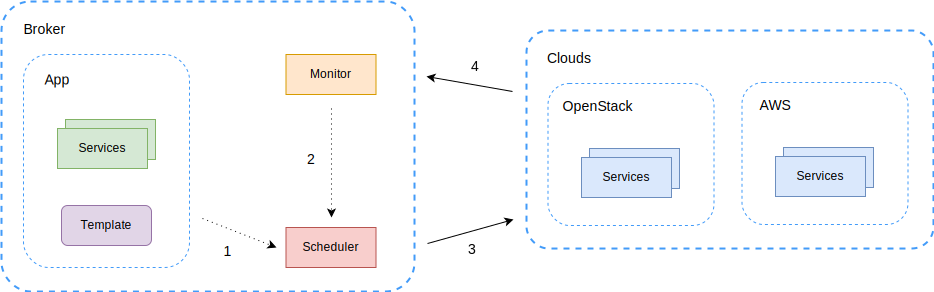
\includegraphics[width=\linewidth]{images/broker-cycle}
	\caption{Arbeitsweise des Multi-Cloud-Brokers als Zyklus: (1) Sammeln der Meta-Informationen alle Cloud-Provider, (2) Sammeln der Laufzeitinformationen der Anwendungen, (3) Sammeln der SLAs, (4) Nutzeränderungen: Neue Anwendungen oder Anpassung von SLAs, (5) Optimierungsplanung, (6) Planausführung auf den Cloud-Infrastrukturen}
	\label{fig:cycle}
\end{figure}

%Zyklus\autoref{fig:cycle}:

%\begin{description}
%	\item[Nummerierte Aufzählung]~\par
\begin{enumerate}
	
	\item Sammeln der Meta-Informationen alle Cloud-Provider
	\begin{enumerate}
		\item Kapazität (CPU, RAM, HDD, Network)
		\item Features (Verschlüsselung, CUDA, …)
		\item Geo-Lokation 
		\item Preis
	\end{enumerate}
	
	\item Sammeln der Laufzeitinformationen der PaaS/Anwendungen
	\begin{enumerate}
		\item Auslastung
		\item Fehler
		\item Ausfälle
	\end{enumerate}
	
	\item Sammeln der SLAs
	\begin{enumerate}
		\item Policy-Definitionen
		\item Policy-Konfiguration
		\item Placement-Algorithmen
	\end{enumerate}
	
	\item Neue Anwendung/Änderung eines SLA
	
	\item Optimierung
	\begin{enumerate}
		\item Feste Vorgaben (Geo, Backup)
		\item Weiche (Preis, Latenz, Verfügbarkeit)
	\end{enumerate}
	
	
	\item Ausführung
	\begin{enumerate}
		\item Netzwerkkonfiguration
		\item Allokation/De-Allokation von Ressourcen
		\item Deployment
		\item Migration
		\item Logging/Benachrichtigung
		\item Backup
	\end{enumerate}
	
\end{enumerate}

\section{Brokering}


%https://de.wikipedia.org/wiki/Constraintprogrammierung
%https://de.wikipedia.org/wiki/Scheduling

%entailing multiple constraint satisfaction (MCS)
%
%\todo{Schaubild, was wird wann gematcht}
%% Pseudocode des Algorithmus, wie in Meryn
%
%Kostenoptimierung
%
%Preisentwicklung? 
%
%Migration je nach Tageszeit? 
%
%Kosten der Datentransfers 
%
%Subscription On-Demand/Monthly/Yearly 
%
%Kompliziert durch undurchsichtige Staffelpreise
% https://www.rightscale.com/blog/cloud-cost-analysis/aws-vs-azure-vs-google-cloud-pricing-compute-instances

%https://www.rightscale.com/blog/cloud-cost-analysis/comparing-cloud-instance-pricing-aws-vs-azure-vs-google-vs-ibm

%
%Cost Calculators 
%
%http://go.appscale.com/cloud-cost-calculator-help 
%
%https://github.com/ifosch/accloudtant 
%
%https://awstcocalculator.com/# 
%

\section{Testumgebung: OpenStack \& Hyrise-R}

Hyrise\footnote{\url{https://hpi.de/plattner/projects/hyrise.html}} ist eine In-Memory-Forschungsdatenbank der Fachgruppe \emph{Enterprise Platform and Integration Concepts (EPIC)} am Hasso-Plattner-Institut \cite{grund:2010:hyrise}. Die Datenbank teilt sich einige Eigenschaften mit \emph{SAP HANA}\footnote{\url{https://www.sap.com/products/hana.html}}: Ein \emph{Delta Store}, spaltenorientierte Speicherung, Wörterbuchkodierung und weitere Komprimierungstechniken sowie den \emph{Insert-Only}-Ansatz und Partitionierung. Herausragend ist die OLAP-Performance, enthalten sind aber auch Optimierungen für OLTP-Aufgaben.

Hyrise-R ist eine Erweiterung des Basisprojektes um Replikation \cite{schwalb:2015:hyrise-r}. Es folgt dabei dem \emph{Scale-Out}-Ansatz: Alle schreibenden Operationen werden auf einem einzigen \emph{Master-Node} durchgeführt. Dessen Datensatz wird in weniger als einer Sekunde (\emph{lazy}) mit beliebig vielen \emph{Replica-Nodes} abgeglichen. Diese Spiegelungen bearbeiten alle reinen Leseanfragen und machen den Verbund so skalierbar, siehe \autoref{fig:hyrise-r}. Nach dem \emph{CAP-Theorem} sind Verfügbarkeit und Partitionstoleranz hier also wichtiger als Konsistenz. 

	\begin{figure}[ht]
	\centering
	\def\svgwidth{0.95\textwidth}
	\includesvg{images/hyrise-r}
	\caption{Verteilte \emph{Hyrise-R}-Architektur mit getrennter Verarbeitung von Lese- und Schreibanfragen. Der Master-Knoten dient als \emph{Single Source of Truth}. Zur Leistungssteigerung übernehmen Spiegelserver die Beantwortung der meisten Leseanfragen. Kleinere Inkonsistenzen werden dabei in Kauf genommen. Aus \cite{ssiclops:d42:experiments-measurements}.}	
	\label{fig:hyrise-r}
\end{figure}

Durch die verteilte Architektur ist Hyrise-R ein potenzieller Kandidat als Testanwendung innerhalb der Multi-Cloud-Umgebung. Einige \emph{SSICLOPS}-Teilprojekte untersuchten bereits Zuverlässigkeit, Performance, Datensicherheit und Vertraulichkeit in einer privaten OpenStack-Föderation \cite{ssiclops:d23:security-extensions, ssiclops:d42:experiments-measurements, bastian:2017:openstack-policies}. \todo{Diagramm:Hyrise-R on SSICLOPS}

Im Rahmen dieser Arbeiten sind einige Infrastrukturteile als Code veröffentlicht: So existiert zum Beispiel eine Docker-Teststellung mit grafischem Cluster-Manager, um die Performance bei verschiedenen Replikationsstufen zu prüfen. Diese Infrastruktur wurde in mehreren Studienarbeiten weiter angepasst, um Hyrise-R-KVM-Images in OpenStack bereitzustellen \cite{eschrig:2016:ssiclops-masterproject, maschler:2017:ssiclops-masterproject}. Möglicherweise können Teile dieser Arbeiten weiterentwickelt werden.


\input{content/4-4_openstack-testbed.tex}

\input{content/4-5_devstack-docker.tex}

\input{content/4-6_multi-cloud-bibliotheken.tex}


\section{Entwicklungsumgebung}

% Hyrise-R-OpenStack- und Docker-Images, wie ersxtellt?

%Bestehende verteilte Anwendungen für den EInsatz in der CLoud vorbereiten, STichwort CLoud Native.
%Ausgangslage? Git-Repository mit teilautmatisierten Shell-Skripten und Makefiles. Automatisierung der Build, Test und Produktions-Infrastruktur, Ubuntu 16.04 auf Bare-Metal, VM und (Docker)Container.
%Integrieren der bestehenden Tests in diese Umgebungen.
%Packen des Geamtpakets aus Ausführungsumgebung, Programm und (Test-)Daten. auch automatisiert. Die Konfiguration ist variabel. SIe wird schematisch in der App-Konfiguration vorgegeben und dann von der CMP während der initialen Bereitstellung oder späteren Re-Deployments angepasst und ausgeführt.

% Tatsächliche Broker Architektur
% Code-Eigenheiten
% Tests/KPIs/Validierung der Hypothese

\section{Softwarearchitektur}

%as in Grozev 42: Federated CLoud Management: There is a central repository of images. this is replicated to the specific iaas/caas providers on demand.
%
%Alle weiteren Managementprozesse sind für Clients transparent.


\section{Multi-Provider-Service-Schema}

% D2.1: Übersicht Policy-Sprachen: Performance und Speichergröße. Entgegengesetzte Interessen. Lesbarkeit über zweiteiliung: Einmal für Menschen, einmal auf Bit-ebene für Maschinen. SLA über Proxy

%D2.2: Policys auf allen Schichten

%Matthias Bastian: Policy in OpenStack.

...und SLAs.

Ziel: Portabilität.

Mensch-und maschinenlesbar

YAML als aktuellen Standard

%TOSCA komplex, aber vielversprechend. Hierauf aufbauen (eigenen YAML-Entwurf erwähnen) und Brokering hinzufügen. Hier muss festgelegt erden, welcher Service-Teil auf welchem Provider mit welchem Instanz-Typen bereitgestellt werden soll. Dies soll automatisiert anhand von SLA/Policy und Preis entschieden werden. Unterstützt TOSCA deklarative Service-Definitionen?
%
%
%TOSCA hat folgendes nur optional
%- YAML (als SimpleVersion)
%- Multi-Provider als Plugin (nicht gewartet)
%- 
\begin{listing}[ht]	
	\inputminted[]{yaml}{./src/provider.sample.yaml}
	\caption{Provider-Definition und Zugangsdaten. Der Broker liest alle eingetragenen Accounts automatisch ein und berücksichtigt sie bei der initialen Service-Bereitstellung sowie in Optimierungsläufen. Public-Clouds benötigen nur Zugangsdaten wie Benutzername und Passwort -- alle weiteren Informationen erfragt der Broker dynamisch zur Laufzeit vom Provider. In Private-Cloud-Umgebungen ist dies nicht immer möglich: Details zur Verfügbarkeit, geografische Lage und Kosten müssen manuell eingepflegt oder vom Monitoring festgestellt werden.}
	\label{listing:provider}
\end{listing}



Platzhalter werden mit Jinja während des Deployments gefüllt.

Ablage der Pläne als Dokumentation.

Broker durch Metainformationen (und Labels) der Instanzen theoretisch zustandslos -> Broker selbst ist nicht ausfallgefährdet.

Erklärung der Metainformationen (versionierbar), verschiedenen Parameter und Rollenbeschreibung.

Je Provider Angaben zu Image und Startkommando. Dies wird hier eingetragen, um vom Broker dynamisch mit aktuellen Variablen angepasst zu werden: IP, Port...

Abhängig vom Service Level: IaaS/CaaS. Auch PaaS ist so denkbar. (Angabe als Image, Interpretation durch den Broker)

Beispiel verlinken.
Kapitel: Legacy Services Hyrise

Image-Erstellung und Repository.

Eigene Befehle
- Cloud-Init (Standard)
- shell/bash (Docker)

Vordefinierte Policys z.B. zum Verhalten im Fehlerfall. Aber auch Zusatzinformationen: Wie ist die Zustandsprüfung auf Service-Ebene auszuführen. Wichtig für Monitoring der Verfügbarkeit (SLA).

Abhängigkeiten von Services und wie oft global vorhanden? Hier: global ein master, abhängig vom Dispatcher.

\begin{listing}[ht]	
	\inputminted[firstline=15]{yaml}{./src/hyrise-r.sample.yaml}
	\caption{Providerübergreifende Servicevorlage. Der Ausschnitt zeigt die Definition des zentralen \emph{Hyrise-R-Dispatcher}-Dienstes. Nicht zu sehen sind Metadaten und die übrigen Anwendungsbestandteile. Parameter werden zur Laufzeit vom Broker eingesetzt.}
	\label{listing:hyrise-r}
\end{listing}

Könnte auch zu einem konkreten CAMP-Plan umgewandelt werden. So wie TOSCAMP. Stattdessen nur ein Template Schema und Graph zur Laufzeit.
%https://brooklyn.apache.org/v/latest/blueprints/setting-locations.html


\section{Tests und Diskussion}

%Kosten: Rechenzeit und Bandbreite (außerhalb einer Cloud) also gegenläufiges Ziel zu Portabilität und Ausfallsicherheit, denn die geringsten Kosten fallen bei dem Betrieb in einer einzelnen Cloud eines Providers an.
%i) providers’ pricing models, (ii) application’s communication patterns and (iii) distribution of nodes over providers.
%https://www.google.de/url?sa=t&rct=j&q=&esrc=s&source=web&cd=1&ved=0ahUKEwju27vHs6DZAhUCWRQKHRv7BEcQFggrMAA&url=http%3A%2F%2Fwww.mikesmit.com%2Fwp-content%2Fpapercite-data%2Fpdf%2Fcloud2012.pdf&usg=AOvVaw3e6yhHYmhWBbIxtr7MqkuX

%verschiedene OpenStack-Versionen haben unterschiedliche Schnittstellen. Auch dies kann über die Middleware abgefangen werden. RefStack testet API, Rally testet performance und führt tempest-Tests aus.


Aufwand einer Multi-Cloud-Strategie

Umsetzung der Policys

Potential

Vorteile durch Multi-Cloud-Bibliotheken

Aufwand für ein Multi-Cloud-Testbed
	\chapter{Test und Diskussion}

\todo{Intro, Motivation, Überblick}

\section{Public-Cloud: AWS-Testbed}
\label{sec:aws-testbed}

\todo{AWS-Intro} Die Amazon-Web-Services-Integration ist eine besondere Herausforderung: Der komplette Auf- und Abbau der Testinfrastruktur benötigt mehrere Minuten. Zusätzlich kostet jede Ressourcennutzung Geld, unabhängig vom Zweck. Zwar stellt Amazon einmalig 100 Dollar Testbudget zur Verfügung; bei mehreren Hyrise-Instanzen sind diese jedoch innerhalb weniger Tage aufgebraucht. Durch die komplexe Struktur der Amazon-Dienste entsteht -- gerade während der Entwicklung des Cloud-Adapters -- ein hohes Kostenrisiko. Der Amazon-Container-Dienst ECS setzt immer eine gestartete Instanz der Elastic Compute Cloud (EC2) voraus. Diese verursacht auch Kosten, wenn kein Container ausgeführt wird. Damit ist das AWS-Verhalten nicht intuitiv und steht in Gegensatz zur \emph{On-Demand}--Philosophie.

Um Aufwand und Risiko zu senken, eignen sich nicht-funktionale Platzhalter-Bibliotheken, sogenannte \emph{Mocks}. Sie implementieren die gleichen Schnittstellen wie herstellereigene Originale und beantworten Anfragen entsprechend -- jedoch ohne tatsächlich eine Netzwerkverbindung und entfernte Ressourcen zu nutzen. Für AWS existieren zwei interessante Projekte; \emph{Moto}\footnote{\url{http://docs.getmoto.org/en/latest/}} und \emph{LocalStack}\footnote{\url{https://localstack.cloud/}}. 

Moto ist eine Python-Bibliothek, die AWS-Aufrufe per Decorator oder Context-Manager direkt im Quellcode umleitet. Der angedachte Anwendungsfall ist die Kombination mit \emph{boto}, dem offiziellen AWS-Python-SDK\footnote{\url{https://aws.amazon.com/de/sdk-for-python/}}.

LocalStack ist  bibliotheks- und programmiersprachen-unabhängig. Es erstellt HTTP-Endpunkte für alle AWS-Dienste. Änderungen im Quellcode der eigentlichen Anwendung sind dafür nicht nötig. Daher ist auch eine Kombination mit Libcloud denkbar, um den Aufwand der AWS-Integration erheblich zu senken. Insgesamt erfordert die Arbeit mit AWS viel Aufmerksamkeit -- die wir lieber in die Konzeption des Brokers investieren. Im lokalen Test- und Entwicklungs-Set-up nutzen wir deshalb Docker als Amazon-ECS-Ersatz.

Für OpenStack sind keine derartig ausgereiften Mock-Projekte bekannt. Alle offiziellen Bibliotheken dienen eher zum Test der OpenStack-Komponenten selbst. Eine tatsächliche Ausführung von Gastanwendungen ist nicht vorgesehen. Um die Funktion mit OpenStack zu validieren, erstellen wir später unser eigenes Testbed im \autoref{sec:openstack-testbed}. Längerfristig wollen wir von Libcloud profitieren, da der Implementierungsaufwand nur einmalig anfällt. Anschließend existiert die Abstraktionsebene unabhängig von potenziellen Schnittstellenänderungen eines Cloud-Providers.

\section{Private-Cloud: OpenStack-Testbed}

Als Beispiel für eine Private-Cloud -- als Teil unseres Multi-Cloud-Setups -- soll OpenStack dienen. Es ist das populärste Open-Source-Projekt um eigene Infrastruktur als Service aufzubauen. Gesponsert wird es von Großunternehmen wie \emph{HPE}, \emph{IBM}, \emph{Canonical}, \emph{Red Hat} und anderen.

OpenStack setzt sich aus verschiedenen Teilprojekten zusammen, die jeweils einen Dienst entwickeln und bereitstellen. Ein Minimal-Setup besteht aus \emph{Nova} (Computing), \emph{Key\-stone} (Authentifizierung), \emph{Neutron} (Netzwerk) und \emph{Glance} (Images). Verbreitet sind außerdem \emph{Cinder} (Blockspeicher) und \emph{Horizon} (Dash\-board). Diese sollen auch in unserem Beispiel genutzt werden. Denkbar ist darüber hinaus die Integration eines Container-Dienstes. Der Zugriff auf die Infrastruktur erfolgt entweder über das Dashboard, Kommandozeilentools oder eine REST-API.

Grundsätzlich wäre auch der Aufbau einer OpenStack-Föderation wie in \emph{SSICLOPS} denkbar \cite{ssiclops:2015:d6.1-project-presentation}. Föderierte Cloud-Architekturen teilen sich zentrale Komponenten, in OpenStack mindestens den Authentifizierungsservice \emph{Keystone}. Je nach Föderationsvariante (\emph{Cells}, \emph{Regions}, \emph{Availability Zones} oder \emph{Host Aggregates}) sind auch Dienste wie Dashboard oder Speicher nur einmal vorhanden. Diese Architektur reduziert Fixkosten, erfordert allerdings spezielle Anpassungen innerhalb der Cloud. Auch gehen einige Vorteile wie Ausfallsicherheit und Unabhängigkeit der zentralen Dienste wieder verloren. Eine Kombination mit weiteren Cloud-Providern im Rahmen unseres Multi-Cloud-Setups ist denkbar, bleibt aufgrund der aufwendigen Einrichtung aber außen vor. Auch wäre der zusätzliche Erkenntnisgewinn vermutlich gering.

Selbst ein minimales OpenStack-Testsetup ist durch die diversen Dienste komplex. Denkbar wäre also auch die Nutzung von externen OpenStack-Angeboten. In diesem Projekt gibt es hierfür grundsätzlich drei mögliche Bereitstellungsmodelle: 

\begin{enumerate}
	\item Public Cloud
	\\\emph{Betrieb auf geteilter Cloud-Infrastruktur}
	
	\item Hosted Private Cloud
	\\\emph{Betrieb auf exklusiver Cloud-Infrastruktur}
	
	\item Lokale Testinstallation
	\\\emph{Betrieb auf eigener physischer oder virtueller Infrastruktur}
\end{enumerate}

\noindent Eine Liste öffentlicher OpenStack-Angebote findet sich auf der Projekthomepage\footnote{\url{https://www.openstack.org/marketplace/hosted-private-clouds/}}. Dort werden auch weitere Informationen wie Funktionsumfang und Zertifizierungen aufgeführt. 

Interessant ist zum Beispiel das Angebot der Deutschen Telekom \emph{Open Telekom Cloud\footnote{\url{https://cloud.telekom.de/en/infrastructure/open-telekom-cloud/}}}: eine Public Cloud auf OpenStack-Basis -- in Deutschland -- mit vollem Funktionsumfang und API-Zugriff. International bietet \emph{Rackspace} eine Hosted Private Cloud\footnote{\url{https://www.rackspace.com/openstack/}}. Beide eignen sich jedoch kaum, um kleine Experimente zu starten, sondern richten sich vor allem preislich an größere Organisationen und Unternehmen.

Kostenlos ist das Public-Cloud-Angebot \emph{TryStack}\footnote{\url{http://trystack.org/}}. Sponsoren wie \emph{Cisco}, \emph{NetApp}, \emph{Dell} und \emph{Red Hat} finanzieren das Projekt. Die Registrierung erfolgt über die Aufnahme in eine Facebook-Gruppe, anschließend soll hierüber auch der Zugang zur kostenlosen OpenStack-\emph{Liberty}-Instanz erfolgen. Während der gesamten Laufzeit dieser Arbeit war allerdings weder ein Login noch Kontakt zu den Organisatoren möglich.

Lokale OpenStack-Installationen sind aufwendig: Für jeden Dienst muss ein eigener physikalischer Rechner bereitstehen. Dementsprechend verweist die offizielle Dokumentation direkt auf die Vielzahl von OpenStack-Distributionen\footnote{\url{https://www.openstack.org/marketplace/distros/}}. Diese bieten fast immer einen vereinfachten Setup-Prozess und oft die Option statt physikalischen Rechnern virtuelle Maschinen oder Container zu nutzen. Wie auch bei den Hosted-Angeboten sind hier nicht alle Dienste verfügbar. In allen Paketen fehlt \emph{Zun}, der aktuelle Container-Service.

Speziell für lokale Test- und Entwicklungsumgebungen existiert \emph{DevStack}\footnote{\url{https://docs.openstack.org/devstack/latest/}}. Das offizielle OpenStack-Projekt installiert automatisiert die wichtigsten OpenStack-Dienste auf einer einzigen Maschine. Ausdrücklich unterstützt werden dabei auch VMs und \emph{LXC}-Container. Es soll daher als Erstes erprobt werden.

\section{DevStack virtualisiert inkl. Container-Support}

Während der Installation nimmt DevStack tief greifende Veränderungen am Hostsystem vor. Es müsste also auf einem separaten Server installiert werden. Dieser Abschnitt beschreibt den Versuch einer virtualisierten, reproduzierbaren DevStack-Testinstallation. Außerdem soll \emph{Zun} integriert werden. 

Ziel ist DevStack in einem Container auszuführen, genauso wie die darin gestarteten Compute-Nodes ebenso in einem -- nun verschachtelten -- Container bereitzustellen. Die Gründe hierfür sind zusammengefasst:

\begin{enumerate}
	\item Keine oder minimale Änderungen am Hostsystem
	\item Reproduzierbarer Testaufbau
	\item Schneller und rückstandsloser Reset
	\item Zustände (\emph{Snapshots}) speicherbar
	\item Schnelle Ausführung von Gastapplikationen
\end{enumerate}

\noindent Auch eine virtuelle Maschine löst die oben genannten Probleme. Theoretisch. Problematisch wird die Ausführungsgeschwindigkeit von Gastanwendungen in einem mit \emph{VirtualBox} virtualisierten OpenStack. Eine Lösung ist \emph{verschachteltes KVM}, das bereits in der Arbeit [1] erprobt wurde. Die Autoren empfehlen ihren Vorschlag bei bestehenden Erfahrungen mit \emph{libvirt}. Der damalige Versuchsaufbau stellt sich allerdings als instabil und nicht mehr reproduzierbar heraus.

\begin{figure}[ht]
	\centering
	\begin{subfigure}[b]{0.29\textwidth}
		\def\svgwidth{\linewidth}
		{\tiny \textsf{
			\includesvg{images/devstack-bare-metal}}}
		\caption{Bare-Metal-Installation}
		\label{fig:sub:devstack-bare-metal}
	\end{subfigure}\hfill%
	\begin{subfigure}[b]{0.31\textwidth}
		\def\svgwidth{\linewidth}
		{\tiny \textsf{
			\includesvg{images/devstack-vm}}}
		\caption{All-in-One-VM}
		\label{fig:sub:devstack-vm}
	\end{subfigure}\hfill%
	\begin{subfigure}[b]{0.31\textwidth}
		\def\svgwidth{\linewidth}
		{\tiny \textsf{
			\includesvg{images/devstack-docker}}}
		\caption{DevStack in Docker}
		\label{fig:sub:devstack-docker}
	\end{subfigure}
	
	\caption{Verschiedene Installationsvarianten für eine OpenStack-Testinstallation mit DevStack auf einem einzelnen Host -- inklusive Unterstützung für Docker-Compute-Container und klassische VMs. Eine direkte Installation verändert unwiderruflich das gesamte Host-System \emph{(a)}. Eine VM benötigt mehr Ressourcen und kann die Geschwindigkeit der Gastanwendungen negativ beeinflussen \emph{(b)}. Die Installation in einem Container schafft Abstraktion und Reproduzierbarkeit ohne Geschwindigkeitskompromisse. Die Gastcontainer nutzen weiterhin den Kernel des Host-OS \emph{(c)}.}
	\label{fig:devstack}
\end{figure}

\emph{LXD}-Container könnten sich ebenfalls eignen. Im Gegensatz zu Docker führen sie mehrere Prozesse aus, erinnern also mehr an eine klassische virtuelle Maschine (ohne deren Overhead). Laut Entwickler \emph{Canonical} fokussiert sich \emph{LXD} speziell auf IaaS-Aufgaben\footnote{\url{https://www.ubuntu.com/containers/lxd}}. Ein LXD-DevStack-Setup birgt allerdings die gleichen Hürden\footnote{\url{https://docs.openstack.org/devstack/latest/guides/lxc.html}} wie ein Docker-Setup \cite{graber:2016:openstack-lxd}. Nennenswert ist noch das OpenStack-Projekt \emph{Kolla}, das jeden OpenStack-Dienst in einem eigenen Docker-Container installiert\footnote{\url{https://cloudbase.it/openstack-kolla-hyper-v/}}.

Um Container innerhalb von OpenStack auszuführen, gibt es mehrere, teils konkurrierende Projekte. Alle lassen sich über Plugins in DevStack einbinden. Zu den Wichtigsten gehören \cite{singh:2017:containers-openstack}:

\begin{description}
	
	\item[Zun\footnotemark]\footnotetext{\url{https://wiki.openstack.org/wiki/Zun}} Eigenständige OpenStack-API zum Starten und Verwalten von diversen Containertypen, inklusive \emph{Docker}.
	
	\item[Nova Docker\footnotemark]\footnotetext{\url{https://wiki.openstack.org/wiki/Docker}} Im Gegensatz zu \emph{Zun} erfolgt die Docker-Containerverwaltung über die bekannte Nova-API. Das Projekt wurde eingestellt.
	
	\item[Nova LXD\footnotemark]\footnotetext{\url{https://linuxcontainers.org/lxd/getting-started-openstack/}} Parallel zu \emph{Nova Docker} erfolgt der Zugriff über die Nova-API. Das Projekt wird von \emph{Canonical} aktiv vorangetrieben. Weiterer Teil ist die Automatisierung via \emph{Juju}.
	
	\item[Magnum\footnotemark]\footnotetext{\url{https://wiki.openstack.org/wiki/Magnum}} Eine Self-Service-Lösung zur Orchestrierung auf Basis von \emph{Heat}. Stellt automatisiert Container Orchestration Engines (COEs) wie \emph{Docker Swarm} und \emph{Kubernetes} bereit.
	
\end{description}

\noindent DevStack in Docker wurde bereits vor einiger Zeit umgesetzt\footnote{\url{https://github.com/ewindisch/dockenstack}}. Da das Projekt nicht mehr gepflegt wird und auf das ebenfalls beendete \emph{Nova Docker} aufsetzt, erfolgt die Neuimplementierung mit folgenden Änderungen:

\begin{itemize}
	
	\item Ubuntu-LTS-Basis-Image 14.04 $\Rightarrow$ 17.10
	\item Mehrprozessunterstützung per \emph{systemd}\footnote{\url{https://docs.openstack.org/devstack/latest/systemd.html}}
	\item OpenStack-Version Kilo $\Rightarrow$ Pike
	\item libvirt/QEMU-Instanzen
	\item Nova Docker $\Rightarrow$ Zun
	\item Container-angepasste DevStack-Konfiguration
	\item Vollständige Netzwerkkonfiguration
	
\end{itemize}

\noindent Größte Hürde ist die Limitierung auf einen Prozess innerhalb eines Standard-Docker-Containers. Neuere DevStack-Versionen setzen auf \emph{systemd}. Daher muss dies über die Umgebungsvariable \emph{ENV container docker} bekannt gemacht werden. Anschließend lässt sich \emph{systemd} über zwei weitere Workarounds starten\footnote{\url{https://github.com/moby/moby/issues/27202}}\footnote{\url{https://github.com/moby/moby/issues/9212}}.

\emph{Docker Build} bereitet das Image mit allen externen DevStack-Abhängigkeiten vor. Notwendige Dienste wie \emph{RabbitMQ} und \emph{MySQL} werden bereits im Voraus installiert. Das Container-Image führt beim Start nur noch die allerletzten Schritte des Setups aus. Ganz vorweg nehmen lässt sich das Setup nicht, weil während des Builds keine erweiterten Rechte vorliegen.

Nach erfolgreichem Start reicht das Kommando \emph{make run}, um per Zun einen \emph{Cirros}-Basis-Container\footnote{\url{https://docs.docker.com/samples/library/cirros/}} zu starten. Der Stand der gesamten OpenStack-Installation lässt sich per \emph{docker commit} oder experimentell per \emph{Docker-Snapshots}\footnote{\url{https://criu.org/Docker}} sichern.

Anpassbar sind im Skript OpenStack-Services und -Versionen, da DevStack direkt aus den Quellen installiert wird. So ändern sich allerdings selbst die Abhängigkeiten der als stabil gekennzeichneten Versionen. Das Prinzip Infrastruktur als Code geht hier nicht immer auf -- DevStack ist nicht zuverlässig reproduzierbar. \autoref{fig:devstack} vergleicht die Installationsvarianten.

Als \emph{Proof-of-Concept} ist die Integration von Docker, DevStack und Zun bisher einmalig. Der Code ist daher auf GitHub\footnote{\url{https://github.com/janmattfeld/DockStack}} veröffentlicht und zeigt einige \emph{Best Practices} und \emph{Lessons Learned} in Bezug auf die genannten Projekte.

Zusätzlich greifen wir auf eine lokale \emph{Mirantis}-OpenStack-Installation aus dem \emph{SSICLOPS}-Projekt zurück. Die Infrastruktur ist virtuell und wird durch \emph{Fuel}\footnote{\url{https://www.mirantis.com/software/openstack/}} zuverlässiger wieder aufgebaut. Die Zun-Container-Dienste sind aufgrund der älteren OpenStack-Version nicht enthalten; dafür aber alle anderen Kernfunktionen und APIs.


\section{Testanwendung: Hyrise-R}
\label{sec:hyrise-r}

Hyrise\footnote{\url{https://hpi.de/plattner/projects/hyrise.html}} ist eine In-Memory-Forschungsdatenbank der Fachgruppe \emph{Enterprise Platform and Integration Concepts (EPIC)} am Hasso-Plattner-Institut \cite{grund:2010:hyrise}. Die Datenbank teilt sich einige Eigenschaften mit \emph{SAP HANA}\footnote{\url{https://www.sap.com/products/hana.html}}: Ein \emph{Delta Store}, spaltenorientierte Speicherung, Wörterbuchkodierung und weitere Komprimierungstechniken sowie den \emph{Insert-Only}-Ansatz und Partitionierung. Herausragend ist die OLAP-Performance, enthalten sind aber auch Optimierungen für OLTP-Aufgaben.

Hyrise-R ist eine Erweiterung des Basisprojektes um Replikation \cite{schwalb:2015:hyrise-r}. Es folgt dabei dem \emph{Scale-Out}-Ansatz: Alle schreibenden Operationen werden auf einem einzigen \emph{Master-Node} durchgeführt. Dessen Datensatz wird in weniger als einer Sekunde (\emph{lazy}) mit beliebig vielen \emph{Replica-Nodes} abgeglichen. Diese Spiegelungen bearbeiten alle reinen Leseanfragen und machen den Verbund so skalierbar, siehe \autoref{fig:hyrise-r}. Nach dem \emph{CAP-Theorem} sind Verfügbarkeit und Partitionstoleranz hier also wichtiger als Konsistenz. 

\begin{figure}[ht]
	\centering
	\def\svgwidth{0.9\textwidth}
	\textsf{
	\includesvg{images/hyrise-r}}
	\caption{Verteilte \emph{Hyrise-R}-Architektur mit getrennter Verarbeitung von Lese- und Schreibanfragen. Der Master-Knoten dient als \emph{Single Source of Truth}. Zur Leistungssteigerung übernehmen Spiegelserver die Beantwortung der meisten Leseanfragen. Kleinere Inkonsistenzen werden dabei in Kauf genommen. Nicht im Bild ist der Dispatcher zur Anfrageverteilung. Aus \cite{ssiclops:d42:experiments-measurements}.}	
	\label{fig:hyrise-r}
\end{figure}

Durch die verteilte Architektur ist Hyrise-R ein potenzieller Kandidat als Testanwendung innerhalb der Multi-Cloud-Umgebung. Einige \emph{SSICLOPS}-Teilprojekte untersuchten bereits Zuverlässigkeit, Performance, Datensicherheit und Vertraulichkeit in einer privaten OpenStack-Föderation \cite{ssiclops:d23:security-extensions, ssiclops:d42:experiments-measurements, bastian:2017:openstack-policies}.

Im Rahmen dieser Arbeiten sind einige Infrastrukturteile als Code veröffentlicht: So existiert zum Beispiel eine Docker-Teststellung mit grafischem Cluster-Manager, um die Performance bei verschiedenen Replikationsstufen zu prüfen. Diese Infrastruktur wurde in mehreren Studienarbeiten weiter angepasst, um Hyrise-R-KVM-Images in OpenStack bereitzustellen \cite{eschrig:2016:ssiclops-masterproject, maschler:2017:ssiclops-masterproject}.

Um als Testanwendung über mehrere Cloud-Ebenen zu dienen, sollte Hyrise-R auf den verbreiteten Hypervisoren, IaaS- und CaaS-Providern ausführbar sein. Aufgrund der Softwarestruktur, als eigenentwickelte \emph{Low-Level-C++-Anwendung}, eignet Hyrise-R sich nicht direkt\footnote{\url{https://cloud.google.com/appengine/docs/flexible/custom-runtimes/}} als Testanwendung für PaaS-Angebote. Hierfür nutzen wir andere Standardsoftware, die auf den üblichen PaaS-Sprachen wie Java, Python oder Node.js aufbaut.

Hyrise-R ist von Anfang an für die Skalierung über externe Broker konzeptioniert. Die bisherigen Arbeiten haben \emph{Standalone-Cluster-Manager} umgesetzt, erst für Docker und später für OpenStack\footnote{\url{https://github.com/DukeHarris/hyrise_rcm}}\footnote{\url{https://github.com/SSICLOPS/openstack-testbed-vm}}. Die nötigen Clusterinformationen werden Hyrise-Instanzen direkt beim Start als Parameter übergeben. Variablen zur Laufzeitumgebung müssen während des Deployments vom Broker ausgefüllt werden: Konkret benötigt Hyrise einen TCP-Port und eine eindeutige Knoten-ID. Über ihre ID registrieren sich Knoten am Dispatcher. Hierzu benötigen sie dessen IP-Adresse und Port -- der Dispatcher muss also immer als Erstes in einem Cluster bereitstehen. Erst dann können Start und Registrierung des Masters erfolgen. Plattformunabhängig ergeben sich folgende Startskripte für einen Hyrise-R-Cluster:

\begin{description}
	
\item[{[1]} Dispatcher] einmal pro Cluster, zentrale Lastverteilung für alle Anfragen
	
\begin{minted}{jinja}
./dispatcher {{dispatcher.port}} settings.json
\end{minted}
	
\item[{[1]} Master] einmal pro Cluster als \emph{Single-Source-of-Truth}, bearbeitet alle Schreibanfragen, gekennzeichnet durch \emph{nodeId=0}
	
\begin{minted}{jinja}
./hyrise \
  --dispatcherurl={{dispatcher.ip}} \
  --dispatcherport={{dispatcher.port}} \
  --nodeId=0 \
  --port={{master.port}}
\end{minted}

\item[{[0-n]} Replica] optional, beliebig viele Instanzen pro Cluster zur Entlastung des Master-Knotens bei Leseanfragen

\begin{minted}{jinja}
./hyrise \
  --dispatcherurl={{dispatcher.ip}} \
  --dispatcherport={{dispatcher.port}} \
  --nodeId={{replica.id}} \
  --port={{replica.port}}
\end{minted}
	
\end{description}

In vorherigen Projekten entwickelte Images für virtuelle Maschinen laufen auf der verbreiteten Hypervisorkombination aus QEMU und KVM. Die Erstkonfiguration erfolgte bisher über direkte SSH-Kommandos an die gestartete virtuelle Maschine. Dies erforderte die Konfiguration von SSH in den VMs und die Verwaltung von Schlüsseln in der CMP. Zusätzlich entstand eine Wartezeit zwischen VM-Startkommando und Erstkonfiguration, die vorherige Projekte durch Polling noch ausdehnten. Eine elegantere Lösung ist \emph{cloud-init}: Die CMP füllt eine Konfigurationsvorlage und schickt es direkt im Startkommando an den Infrastruktur-Provider. Dieser führt das Skript ohne weitere Wartezeit aus.

Auch Docker-Images existieren bereits unverändert seit 2015\footnote{\url{https://github.com/hyrise/hyrise-v1/tree/feature/docker}}. In der Zwischenzeit wurden Docker, diverse Abhängigkeiten und Hyrise selbst allerdings weiterentwickelt. Innerhalb eines Clusters sollten alle Knoten dieselbe Hyrise-Version ausführen. Daher aktualisieren wir Dispatcher und Hyrise auf Basis des aktuellsten Hyrise-NVM-Branches\footnote{\url{https://github.com/janmattfeld/dispatcher/tree/docker}}\footnote{\url{https://github.com/janmattfeld/hyrise_nvm/tree/feature/docker}}.

Die Aktualisierung enthält das aktuelle Docker-Basis-Image Ubuntu\,16.04. Wir integrieren außerdem korrekte Metadaten und Dokumentation zur Imageerstellung und Ausführung. Einige eingebundene Git-Submodule wurden in der Zwischenzeit verschoben oder existieren nicht mehr -- die verwendete CSV-Bibliothek muss zum Beispiel ausgetauscht werden. Dies erfordert kleinere Änderungen am Quellcode. Genauso wie neue \emph{Non-Uniform-Memory-Access-Funktionen (NUMA)}: Die Funktion \emph{membind} erfordert erweitere Rechte. In einem Standard-Docker-Container sind diese aber nicht vorhanden. Der neue Startparameter \mbox{\emph{-\,-disable\_membind}} deaktiviert die speziellen NUMA-Funktionen. Unsere Images laufen daher auch in Container-Laufzeitumgebungen der Public-Cloud-Provider.

Das Image ist zum Produktivbetrieb gedacht: Docker Build entfernt nach dem Image-Erstellungsprozess alle Abhängigkeiten, die zum Betrieb nicht notwendig sind. So reduziert sich die Image-Größe von über 500 auf weniger als 300\,MB -- entsprechend verkürzt sich die Startzeit. Enthalten ist außerdem eine Beispieldatenbank, die wir später als Benchmark und initialen Funktionstest nutzen werden. Gemessen wird also nicht die Synchronisationszeit der Hyrise-R-Lösung, sondern die Skalierungsfähigkeiten der verwendeten Cloud-Lösungen und Orchestrierungstechniken. Wir setzen außerdem pragmatische Startparameter für Hyrise-R auf Docker: \emph{-\,-corecount=2} \emph{-\,-disable\_membind}. Die neuen Images sind zur leichteren Integration auf Docker Hub veröffentlicht\footnote{\url{https://hub.docker.com/r/hyrise/dispatcher/}}\footnote{\url{https://hub.docker.com/r/janmattfeld/hyrise_r/}}. Um auch zukünftige Weiterentwicklungen von Hyrise nutzen zu können, automatisiert ein neues Makefile Docker-Build-Voränge und den Realease auf Docker Hub.

\begin{figure}[ht]
	\centering
	\begin{subfigure}[b]{0.45\textwidth}
		\def\svgwidth{\linewidth}
		{\scriptsize \textsf{
				\includesvg{images/hyrise-r-runtime-vm}}}
		\caption{Virtuelle Maschine}
		\label{fig:sub:hyrise-r-runtime-vm}
	\end{subfigure}\hfill%
	\begin{subfigure}[b]{0.45\textwidth}
		\def\svgwidth{\linewidth}
		{\scriptsize \textsf{
				\includesvg{images/hyrise-r-runtime-docker}}}
		\caption{Container}
		\label{fig:sub:hyrise-r-runtime-docker}
	\end{subfigure}	
	\caption{Aktualisierte Ausführungsumgebungen für Hyrise-R-Master/Replica auf IaaS- und CaaS-Plattformen. Die Anmerkungen auf der linken Seite beschreiben verwendete Technologien und Schnittstellen.}
	\label{fig:hyrise-r-runtimes}
\end{figure}

Aus der bisher losen Sammlung von Quellcode, Shell-Skripten und Makefiles in mehreren GitHub-Repositorys haben wir eine nachhaltige Pipeline zur automatisierten Image-Erstellung für verschiedene Infrastrukturen entwickelt\footnote{\url{https://github.com/janmattfeld/hyrise_nvm/commit/cfe3aa8}}. Ausführungsumgebung, Programm, Testdaten und Konfiguration werden flexibel integriert -- Hyrise-R eignet sich nun als Testanwendung für den Multi-Cloud-Broker.

Als Weiterentwicklung zu den bisherigen Hyrise-R-Arbeiten soll der Broker nicht nur nach Leistungsanforderungen skalieren, sondern auch SLAs und Geostandorte beachten sowie diverse Infrastrukturanbieter nutzen.


\section{Praxis: Multi-Cloud-Brokering}
\label{sec:brokering-test}

In den vorherigen Abschnitten haben wir die Funktionsweise des Brokers erläutert, den modularen Vorschlag als Python-Service implementiert, sowie Hyrise-R zum Cloud-Betrieb vorbereitet. Auf dem virtualisierten OpenStack-Testbed soll nun die Funktionsweise des Gesamtsystems geprüft werden: Zwei Hyrise-R-Cluster laufen über zwei Clouds verteilt und werden dynamisch skaliert, siehe \autoref{fig:hyrise-r-deployment}.

\begin{figure}[ht]
	\centering
	\def\svgwidth{0.85\textwidth}
	{\scriptsize \textsf{
			\includesvg{images/hyrise-r-deployment}}}
	\caption{Testarchitektur mit zwei Hyrise-R-Clustern, verteilt auf eine Public- und eine Private-Cloud. Cluster \emph{B} nutzt AWS, um unkritische Daten kostengünstig auszulagern. Orchestriert werden beide Services durch die selbst entwickelte Cloud-Management-Plattform aus der Private-Cloud heraus -- die CMP harmonisiert Provider- und Infrastrukturgefälle.}	
	\label{fig:hyrise-r-deployment}
\end{figure}

Wir starten Hyrise-R immer als Cluster aus Dispatcher, Master und einer per SLO-Vorlage bestimmten Anzahl an Replika. Anschließend skalieren wir den Cluster dynamisch nach Leistungsanforderungen und SLO-Bedingungen. Das erneute Starten anhand von veränderter Umgebung ist eingeschränkt: Hyrise-R unterstützt keine Echtzeitmigration. Einzig die Replika lassen sich ohne Probleme an- und abmelden -- für Tests des Cloud-Burstings, also dem Abfangen erhöhter Last durch weitere Instanzen, ist das kein Problem. Entweder der Broker sucht eine passende Infrastruktur und startet einen neuen Hyrise-R-Replika-Knoten, oder er fährt einen Knoten herunter und meldet ihn ab. Die Tests sind rein qualitativ und decken folgende Fälle ab:

\begin{enumerate}
	\item Betrieb über Cloud-Grenzen hinweg
	\item Betrieb auf heterogener Infrastruktur
	\item Skalieren nach Leistungsanforderungen
	\item Skalieren nach weiteren SLOs und Nutzeranforderungen
\end{enumerate}

In einem funktionsfähigen Hyrise-R-Cluster empfängt der Dispatcher alle Anfragen. Jede Anfrage mit Schreibanteil leitet er an den Master-Knoten. Hier wird die Anfrage bearbeitet, in das Log geschrieben und anschließend mit allen Replika synchronisiert. Enthält eine Anfrage nur Leseanteile, verteilt der Dispatcher sie an einen beliebigen Knoten. Frühere Arbeiten bewerteten an dieser Stelle die Anfrageperformance und den Synchronisationsoverhead. Beide Metriken sind jedoch stark abhängig von der Performance der Cloud-Infrastruktur und Netzwerkverbindungen.

Als Metrik zur Bewertung des Brokerings gilt -- neben Einhaltung der SLOs -- die volle Funktionsfähigkeit des Clusters. Eine Beispieldatenbank ist bereits in den Images enthalten. Alle Anfragen haben ausschließlich lesende Anteile, die Tabelle wird nicht durch Schreibanfragen verändert und muss deshalb nicht synchronisiert werden. Gemessen wird also nicht die Synchronisationszeit der Hyrise-R-Lösung, sondern die Skalierungsfähigkeiten der verwendeten Cloud-Lösungen und Orchestrierungstechniken.

Die Hyrise-HTTP-Schnittstelle empfängt Anfragen im JSON-Format. Die minimale Anfrage \emph{NoOp} startet keine Datenbankoperation, durchläuft aber alle Datenbankkomponenten von HTTP-Handling über Parser bis Ausführungseinheit. Als erster Funktionstest würde diese Anfrage genügen. Wir möchten allerdings den gesamten Cluster testen, und nutzen daher eine echte, hinreichend komplexe Anfrage. Deren Bearbeitung benötigt genug Zeit, damit der Dispatcher sie auf alle Knoten aufteilen kann. Den vorhandenen Python-Code überarbeiten und parallelisieren wir. Die Anzahl der Knoten lässt eine bestimmte Performance erwarten -- für einen gültigen Test muss die Anzahl der Anfragen mindestens der Anzahl Knoten entsprechen:

\begin{minted}{python3}
queries = [(host, port, query)] * num_nodes
start_time = time.time()
with multiprocessing.dummy.Pool(num_threads) as pool:
	pool.starmap(query_hyrise, queries)
queries_second = num_nodes / (time.time() - start_time)
\end{minted}

Um sowohl OLTP- als auch OLAP-Fähigkeiten der In-Memory-Datenbank zu überprüfen, nutzen vorherige Arbeiten \cite{ssiclops:d42:experiments-measurements} den CH-benCHmark der TU München \cite{cole:2011:db-benchmark}. Dieser ist eine Mischung aus Transaktions- und Analysebenchmark, angelehnt an den hybriden Einsatz aktueller Datenbanksysteme in Unternehmen: Die gleichen Tabellen eines einzigen Datenbanksystems erfüllen alle Aufgaben des täglichen Geschäfts und liefern gleichzeitig umfassende Analysen. Trotzdem bleibt die Vergleichbarkeit des Benchmarks mit klassischen, getrennten Systemen.

Die Beispieldatenbank enthält eine Auftragshistorie mit knapp 300\,000 Datensätzen. Jede Zeile besteht aus sieben zufälligen Integer-, zwei String- und einem Float-Wert. So ergibt sich eine Rohgröße von 21,3\,MB. Die folgende Beispielanfrage\footnote{\url{https://db.in.tum.de/research/projects/CHbenCHmark/}} zeigt alle Bestellungen eines bestimmten Zeitraumes, sowie Summe, Gesamt- und Durchschnittswert aller enthaltenen Posten. Sie dient uns als \emph{Smoke-Test} -- liefert der Hyrise-R-Cluster eine valide Antwort im vorgegebenen Zeitrahmen, ist die generelle Funktionsfähigkeit gegeben, und das Deployment erfolgreich abgeschlossen:

\begin{minted}{sql}
SELECT ol_number,
       SUM(ol_quantity) AS sum_qty,
       SUM(ol_amount)   AS sum_amount,
       AVG(ol_quantity) AS avg_qty,
       AVG(ol_amount)   AS avg_amount,
       COUNT(*)         AS count_order
FROM orderline 
WHERE ol_delivery_d > '2007-01-02 00:00:00.000000' 
GROUP BY ol_number
ORDER BY ol_number
\end{minted}

%To-do: Konkreter Test, SLOs: Verlinken aus vorherigem Abschnitt. Forschungshypothese: Steigerung von  Datensicherheit, Vertraulichkeit und Portabilität.

\noindent
Das folgende Minimalbeispiel ist der Smoke-Test unseres Prototyps:
\begin{minted}{python}
init_clouds(filter=['ecs', 'openstack'])
deploy_app('hyrise')
validate_throughput('hyrise')
teardown(filter='all')
\end{minted}

\noindent
Um die, in \autoref{cha:implementierung} vorgestellten, Strategien zu Platzierung und anschließender Skalierung zu überprüfen, definieren wir zwei umfangreichere Testfälle, siehe \autoref{tab:testcases}. Der gerade diskutierte Hyrise-R-Benchmark dient dabei zur Bestimmung der Durchsatz-Qualitätsvereinbarung. Gleichzeitig nutzen wir alle definierten Komponenten des Brokers sowie unsere kombinierten Anwendungs- und SLA-Vorlagen.

\begin{table}[h!]
\centering%
\caption{Testfälle der beiden zentralen Broker-Funktionen.}
\ra{1.3}
\begin{tabularx}{\textwidth}{LLLLL}%
\toprule%
%
Test Case & Clouds & Policies & SLAs & Optimization\\%
%
\midrule%
%
Placement & OpenStack, AWS ECS & Geo, Replication & -- & Pricing\\%
Scaling   & OpenStack, AWS ECS & Geo, Replication, Workload & Throughput & Pricing\\%
\bottomrule%
\label{tab:testcases}
\end{tabularx}
\end{table}

Wir haben damit erfolgreich eine interaktive, verteilte Anwendung dynamisch auf verschiedenen Clouds mehrerer Provider verteilt. Dabei beachten wir Qualitätsvereinbarungen und greifen auf Metadaten wie Geo-Standorte und aktuelle Preise zu. Mit dieser Kombination ist der Multi-Cloud-Broker in seinem Forschungsumfeld einzigartig. Welche Stärken und weitere Herausforderungen der Test zeigt, diskutiert der nächste Abschnitt.


\section{Stärken und Herausforderungen}

%verschiedene OpenStack-Versionen haben unterschiedliche Schnittstellen. Auch dies kann über die Middleware abgefangen werden. RefStack testet API, Rally testet performance und führt tempest-Tests aus.


Aufwand einer Multi-Cloud-Strategie

Umsetzung der Policys
- Apps gemeinsam betrachten und optimieren
- Services gemeinsam betrachten und optimieren

Potenzial

Vorteile durch Multi-Cloud-Bibliotheken

Aufwand für ein Multi-Cloud-Testbed

Redundanz fehlt: Auch die CMP muss in einer vertrauenswürdigen Umgebung repliziert werden und synchronisieren. Dem Hyrise-R-Dispatcher fehlt diese Funktion ebenso.

% See IETF Inter Cloud Framework Requirements and Diagram S.26
%Cloud Services Layers (Logical) (Intercloud Communication)
	\chapter{Zusammenfassung und Ausblick}

Cloud-Angebote spielen eine entscheidende Rolle in den aktuellen und zukünftigen IT-Strategien von Unternehmen aller Größen. Besonders attraktiv sind die höhere Flexibilität und mögliche Kosteneinsparungen. Gleichzeitig entstehen größere Herausforderungen bei Zuverlässigkeit und Vertraulichkeit sowie Portabilität der eigenen Daten und Anwendungen. Mit dem Inkrafttreten der Datenschutz-Grundverordnung und immer neuen Datenlecks\footnote{\url{https://www.mcafee.com/enterprise/en-us/solutions/lp/cloud-security-report-stats.html}} ist das Thema hochaktuell.

Durch die Nutzung mehrerer Anbieter und der intelligenten Kombination von Private- und Public-Cloud-Infrastruktur möchten wir diesen Herausforderungen entgegentreten. Cloud-Kunden müssen in der Lage sein, ihre Anforderungen anbieter- und technikunabhängig zu formulieren. Eine technische Lösung sollte anschließend automatisiert die Einhaltung von geforderten Datenschutz-, Qualitäts- und Kostenzielen sicherstellen.

Wir haben einen Überblick über aktuelle kommerzielle und akademische Multi-Cloud-Projekte gegeben. Dabei haben wir fehlende SLA- und Cloud-Schnittstellen-Standards als größte Risiken identifiziert. Als Lösungsvorschlag entwickelten wir einen Multi-Cloud-Broker und implementierten ihn prototypisch. Dabei diente das bestehende TOSCA-Simple-Schema zur Anwendungs- und SLA-Spezi\-fi\-ka\-tion. Die Leistungsfähigkeit der Lösung haben wir anschließend in einem Testaufbau mit OpenStack, AWS und Hyrise-R demonstriert.

Innerhalb von zwei zentralen Testfällen platzieren wir einen Hyrise-R-Cluster über Technik- und Anbietergrenzen hinweg: Dabei beachten wir einfache Regeln zur Redundanz, aber auch komplexere Qualitätsvorgaben wie einen bestimmten Anfrage-Durchsatz. Zusätzlich sind dem Broker Geostandorte der Rechenzentren bekannt, er berücksichtigt also auch aktuelle Datenschutzvorschriften. Abschließend wählt er den kostengünstigsten Anbieter, der alle übrigen Kriterien erfüllt. Dieses Leistungsspektrum macht das Konzept einzigartig und auch kommerziell interessant.

Während Verwaltung und Betrieb verteilter Cloud-Anwendungen deutlich vereinfacht oder sogar erst ermöglicht wurden, ergaben sich größere Herausforderungen bei der Integration verschiedener Cloud-Provider. Besonders Public-Cloud-Angebote wie AWS können sich als Kostentreiber herausstellen, da keine besonderen Rabatte für einen Testbetrieb existieren. Kostengünstiger, aber technisch aufwendiger ist die Bereitstellung eines aussagekräftigen Private-Cloud-Testbeds mit OpenStack. Für beide Fälle haben wir Automatisierungen mithilfe von Platzhaltern und Containern vorgestellt. Von einem Einsatz der Multi-Cloud-Bibliothek Libcloud müssen wir abraten -- statt der erhofften Harmonisierung verschiedener Schnittstellen und Leistungsklassen, bringt die Drittbibliothek einige neue Fehlerquellen.

Insgesamt entsteht aber eine größere Unabhängigkeit von einem einzelnen Cloud-Anbieter. Zusätzlich zur sichergestellten Vertraulichkeit und möglichen Preisvorteilen ergeben sich weitere Vorteile:

\begin{description}
	
	\item[Notfallplan] Bei Ausfall der gesamten Ausführungsplattform kann eine Migration zu einem anderen Anbieter erfolgen.
	
	\item[Abfangen von Lastspitzen] Zusätzliche Service-Instanzen auf externen Ressourcen bearbeiten bei Bedarf weitere Anfragen (\emph{Cloud-Bursting}).
	
	\item[Lebenszyklus-Verwaltung] Typischerweise durchläuft eine neue Anwendungsversion die Phasen Entwicklung, Test, Qualitätssicherung und Produktion. Hierfür existieren oft unterschiedliche Ausführungsumgebungen, die wir automatisiert ansprechen.
	
\end{description}

Während die Portierung bestehender Anwendungen und die Definition der Dienste und SLAs weit fortgeschritten ist, ergeben sich weitere Anforderungen für den produktiven Einsatz als CMP: Aktuell besitzt der Broker keinerlei Authentifizierung, auch eine grafische Anzeige fehlt. Denkbar wäre auch ein Discovery-Dienst wie Zookeeper zur einfacheren Verwaltung der verteilten Anwendungen.

Weitere Forschungsmöglichkeiten existieren vor allem in Bezug auf das Brokering: Möglich sind die Einführung von vertikaler Skalierung, Beachtung von Staffelpreisen und die Optimierung mehrerer Anwendungen gleichzeitig. Eine Lastverteilung auf Datenebene findet aktuell nicht statt, damit bietet das Projekt allerdings eine gute Ergänzung zu den bisherigen Beiträgen im SSICLOPS-Kontext.
	
	% Bibliographie
	\ifisbook\cleardoubleemptypage\fi
	\phantomsection\addcontentsline{toc}{chapter}{\refname}
	\printbibliography[category=cited]

	% Eigenständigkeitserklärung
	\ifisbook\pagestyle{plain}\cleardoubleemptypage\include{content/disclaimer}\fi

\end{document}